\documentclass[tikz, border=10pt]{standalone}
\usetikzlibrary{patterns}
\usepackage[outline]{contour}
\contourlength{0.09em}

\tikzset{
  nodeAll/.style={draw, rounded corners=3pt, text width=1.5em, align=center, thick},
  nodeA/.style={fill=black, text=white},
  nodeB/.style={fill=white, text=black, pattern=north east lines}
}

\begin{document}

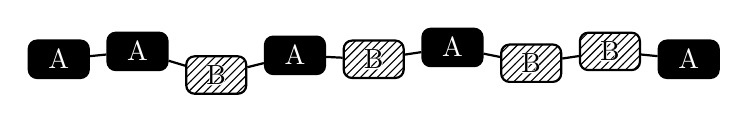
\begin{tikzpicture}
  \node[nodeAll, nodeA] (SC-5) at (-5,0) {A};
  \node[nodeAll, nodeA] (SC-4) at (-4,0.1) {A};
  \node[nodeAll, nodeB] (SC-3) at (-3,-0.2) {\contour{white}{B}};
  \node[nodeAll, nodeA] (SC-2) at (-2,0.05) {A};
  \node[nodeAll, nodeB] (SC-1) at (-1,0) {\contour{white}{B}};
  \node[nodeAll, nodeA] (SC0) at (0,0.15) {A};
  \node[nodeAll, nodeB] (SC1) at (1,-0.05) {\contour{white}{B}};
  \node[nodeAll, nodeB] (SC2) at (2,0.1) {\contour{white}{B}};
  \node[nodeAll, nodeA] (SC3) at (3,0) {A};

  \path[thick]
    (SC-5) edge (SC-4)
    (SC-4) edge (SC-3)
    (SC-3) edge (SC-2)
    (SC-2) edge (SC-1)
    (SC-1) edge (SC0)
    (SC0) edge (SC1)
    (SC1) edge (SC2)
    (SC2) edge (SC3);
\end{tikzpicture}
\end{document}
